%%%%%%%%%%%%%%%%%%%%%%%%%%%%%%%%%%%%%%%%%%%%%%%%%%%%%%%%%%%%%%%%%%%%%%%%%%%%%%%
% NAME:             server-arch.tex
%
% AUTHOR:           Ethan D. Twardy
%
% DESCRIPTION:      Design Document for the Server Architecture.
%
% CREATED:          07/02/2018
%
% LAST EDITED:      07/04/2018
%%%

\documentclass[12pt]{article}
\pagestyle{empty} % Prevent style conflicts with `fancy'
\usepackage[margin=1in]{geometry} % Pretty much just to set the margins
\usepackage{fancyhdr} % Header & Footer
\usepackage{setspace} % Spacing.
\usepackage{graphicx}

\title{Server Architecture Design Document}
\author{Ethan D. Twardy}

% Header
% pdflatex will probably complain about \headheight.
%% \setlength{\headheight}{28pt}
\pagestyle{fancy}
\fancyhf{}
% Header
\rhead{Ethan D. Twardy}
\lhead{\title}

% This may come in handy.
%% \setlength{\emergencystretch}{15pt}
\setlength{\parskip}{10pt}
\setlength{\parindent}{0pt}

\begin{document}
\maketitle
\pagebreak

% TODO: Make toc

\section{Block Diagram}
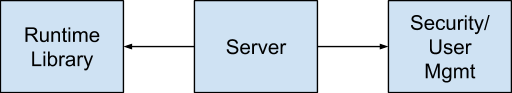
\includegraphics[width=\textwidth]{arch.png}

\section{Server}
This module is responsible for managing network connections with clients,
authenticating users, and facilitating the use of the Autoscrum system. This
module communicates directly with the Autoscrum Runtime Library and the
Security and User Management modules on behalf of the Client.

\section{Client (Not Shown)}
This module receives input from the user and communicates with the Server
module to service user requests. This module is not shown in the block diagram.

\section{Runtime Library}
This module implements the Autoscrum object management logic. For example, this
module manages all Autoscrum objects in the system, and facilitates
relationships between these objects. This module exports a complex API meant to
be utilized by a server/client implementing an Autoscrum system.

\section{Security/User Management}
This module is responsible for controlling access to particular objects in the
Autoscrum ecosystem. This module is an implementation independent adaptor for
preexisting security systems. Since it is most likely going to be a
particularly volatile module, it shall have no prior dependencies, and its
interface shall be frozen.

\end{document}

%%%%%%%%%%%%%%%%%%%%%%%%%%%%%%%%%%%%%%%%%%%%%%%%%%%%%%%%%%%%%%%%%%%%%%%%%%%%%%%
